%!TEX root = ../thesis.tex

\thispagestyle{myheadings}

\graphicspath{{Body/Figures/Wa/Datasets/Endgame/LostMuonFiles/MainCuts/}{Body/Figures/Wa/Datasets/ComparisonPlots/LostMuons/}{Body/Figures/Wa/Datasets/9d/SingleIteration/LostMuonFits/}{Body/Figures/Wa/Datasets/9d/PileupJobs/PileupGapTime/}{Body/Figures/Wa/Datasets/9d/PileupJobs/PileupDeadTime/auto-scaling/}{Body/Figures/Wa/Datasets/9d/PileupJobs/PileupDeadTime/fixed-scaling/}{Body/Figures/Wa/Datasets/9d/PileupJobs/PileupEnergyScale/}{Body/Figures/Wa/Datasets/9d/PileupJobs/PileupTimeShift/}{Body/Figures/Wa/Datasets/9d/SingleIteration/PileupMultiplierScan/}{Body/Figures/Wa/Datasets/60h/RatioConstruction/Ta/}{Body/Figures/Wa/Datasets/60h/RatioConstruction/TauMu/}{Body/Figures/Wa/Datasets/9d/Binning/BinEdge/}{Body/Figures/Wa/Datasets/9d/Binning/BinWidth/}{Body/Figures/Wa/Datasets/60h/Gain/0p25-steps/}}




\section{Systematic errors}
\label{sec:Systematic Errors}



\begin{table}[]
\centering
\setlength\tabcolsep{10pt}
\renewcommand{\arraystretch}{1.2}
\begin{tabular*}{.8\linewidth}{@{\extracolsep{\fill}}lc}
  \hline
    \multicolumn{2}{c}{\textbf{\wa Measurement Uncertainties}} \\
  \hline\hline
    Source of uncertainty & E989 Goal (ppb) \\
  \hline
    Gain changes & 20 \\
    Pileup & 40 \\
    Lost muons & 20 \\
    CBO & 30 \\
    E field and pitch corrections & 30 \\
  \hline
    Quadrature sum & 70 \\
  \hline 
\end{tabular*}
\caption[Uncertainties in the precession frequency measurement]{Systematic errors in the precession frequency measurement. \textbf{fill this table out more once I've gone through the various parts - mention that this is the final expected table}}
\label{tab:wauncertainties}
\end{table}





\subsection{Pileup systematic errors}
\label{sub:pileuperror}

As described in \secref{sub:pileupsubtraction}, the pileup background oscillates at \wa which by extension means a strong effect on the final fitted $R$ value. If the subtracted pileup spectrum is mis-constructed in any way, there will be a systematic error on $R$. In general the pileup systematic error can be separated into two parts, the error on the amplitude and the error on the phase. In order to estimate the two parts, the uncertainties on the pileup amplitude and phase need to be estimated along with the sensitivities of $R$ to them. \tabref{tab:histogramparameters} gives the default values used for the pileup construction parameters \{ADT, SDT, SGT, C\}. How these parameters feed into the amplitude and phase systematic errors will be discussed in turn, and the overall errors calculated for the different Run~1 datasets.


As a reminder the default values used for the ADT and SDT were \ns{5} each, and a default automatic pileup amplitude multiplier of $\sim1.03$ was applied to the pileup spectra. In order to calculate the systematic dependence on the choice of ADT or SDT, the SDT parameter was scanned over from \ns{5} to \ns{10} in steps of \ns{1}. This was done with and without the same automatic pileup amplitude scaling procedure as described in \secref{sub:pileupsubtraction}. The results of the study for the 9d dataset are shown in Figures~\ref{fig:SDTscan_noScaling} and \ref{fig:SDTscan_autoScaling}. In the case where there was no automatic scaling applied there is a clear minimum in the \chisq results and a steep slope in $R$ corresponding to a large sensitivity of $R$ to the choice of SDT. In the case where the automatic scaling was applied however, the minimum in the \chisq results has disappeared, while the sensitivity of $R$ has become much reduced to the point of no longer being a clear trend\footnote{This slope in $R$ varies between positive and negative values based on dataset, so there is no real clear trend in $R$.}. The fact that applying the automatic pileup amplitude scaling produces nearly identical pileup spectra with no clear trend in $R$ regardless of the choice of SDT (and by extension ADT), any systematic error due to the choice of these two parameters can be subsumed into the direct pileup amplitude error itself, discussed down below. It should be noted in fact that the choices of ADT and SDT are largely irrelevant barring statistics, as the automatic amplitude scaling procedure can always account for any differences between the two. 


\begin{figure}[]
\centering
    \begin{subfigure}[t]{0.45\textwidth}
        \centering
        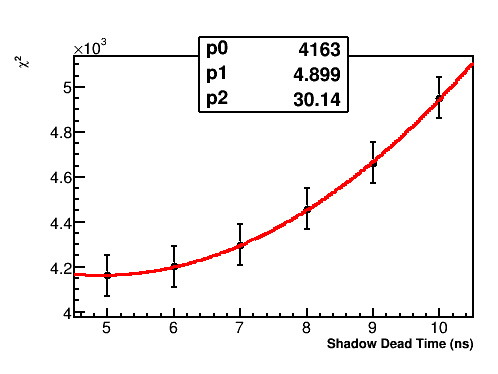
\includegraphics[width=\textwidth]{FullRatio_Chi2_Vs_ShadowDeadTime_Canv_9d_fixed}
        \caption{\chisq versus SDT. The parabolic fit equation used was $y = p_{2}(x - p_{1})^{2} + p_{0}.$}
    \end{subfigure}% %you need this % here to add spacing between subfigures
    \hspace{1cm}
    \begin{subfigure}[t]{0.45\textwidth}
        \centering
        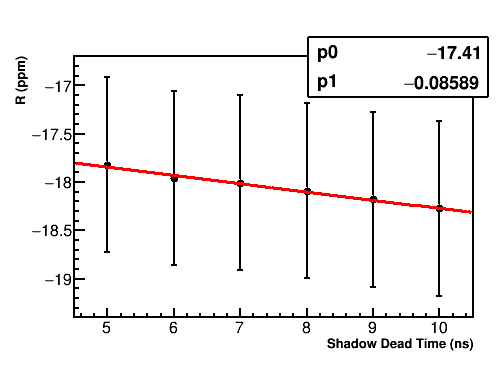
\includegraphics[width=\textwidth]{FullRatio_R_Vs_ShadowDeadTime_Canv_9d_fixed}
        \caption{$R$ versus SDT. The parameter $p_{1}$ gives the sensitivity of $R$ to the value of SDT, with units in ppm/ns.}
    \end{subfigure}

    \begin{subfigure}[t]{0.45\textwidth}
        \centering
        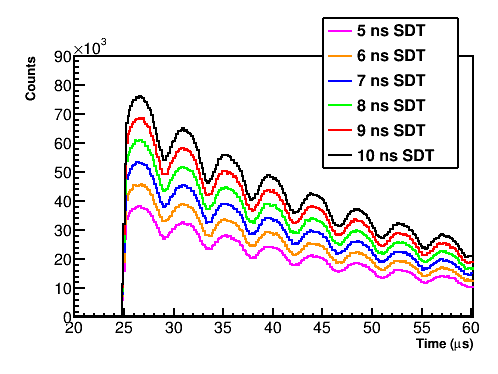
\includegraphics[width=\textwidth]{SDT_PileupTimeComparison_9d_fixed}
        \caption{The pileup time spectrum for different choices of SDT.}
    \end{subfigure}% %you need this % here to add spacing between subfigures
    \hspace{1cm}
    \begin{subfigure}[t]{0.45\textwidth}
        \centering
        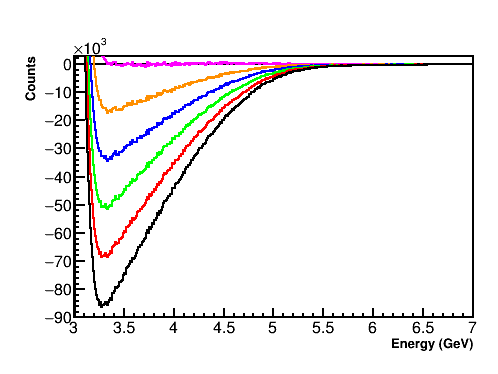
\includegraphics[width=\textwidth]{SDT_CorrEnergyComparison_9d_fixed}
        \caption{The corrected energy spectrum for different choices of SDT.}
    \end{subfigure}
\caption[Pileup shadow dead time scan without automatic pileup amplitude scaling]{Shadow dead time scan results without automatic pileup amplitude scaling. A clear minimum in the \chisq plot is seen near \ns{5} corresponding to the choice of ADT, and a large sensitivity for $R$ is observed. In the bottom two spectra plots the magenta curve corresponds to a choice SDT = \ns{5} while the black curve corresponds to SDT = \ns{10}. The larger choice of SDT leads to a greater estimation of the pileup, which as shown in the energy spectra plot leads to a corresponding over-subtraction at energies where hits consist mostly or purely of pileup pulses. Data from 9d dataset.}
\label{fig:SDTscan_noScaling}
\end{figure}


\begin{figure}[]
\centering
    \begin{subfigure}[t]{0.45\textwidth}
        \centering
        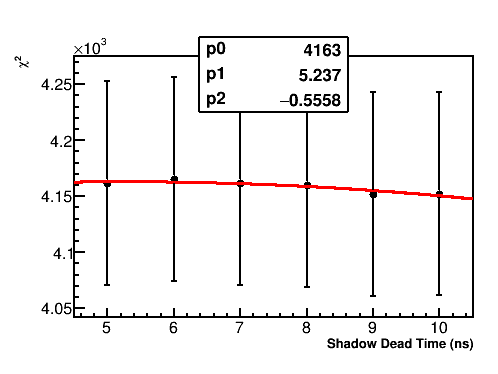
\includegraphics[width=\textwidth]{FullRatio_Chi2_Vs_ShadowDeadTime_Canv_9d_auto}
        \caption{\chisq versus SDT. The parabolic fit equation used was $y = p_{2}(x - p_{1})^{2} + p_{0}.$}
    \end{subfigure}% %you need this % here to add spacing between subfigures
    \hspace{1cm}
    \begin{subfigure}[t]{0.45\textwidth}
        \centering
        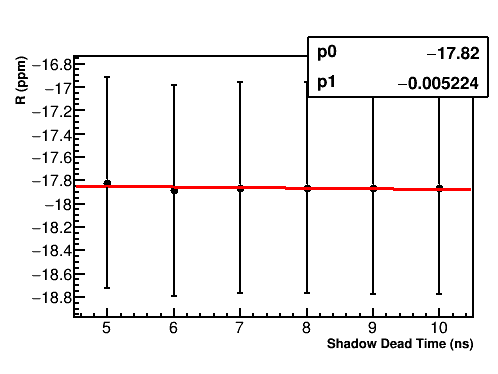
\includegraphics[width=\textwidth]{FullRatio_R_Vs_ShadowDeadTime_Canv_9d_auto}
        \caption{$R$ versus SDT. The parameter $p_{1}$ gives the sensitivity of $R$ to the value of SDT, with units in ppm/ns.}
    \end{subfigure}

    \begin{subfigure}[t]{0.45\textwidth}
        \centering
        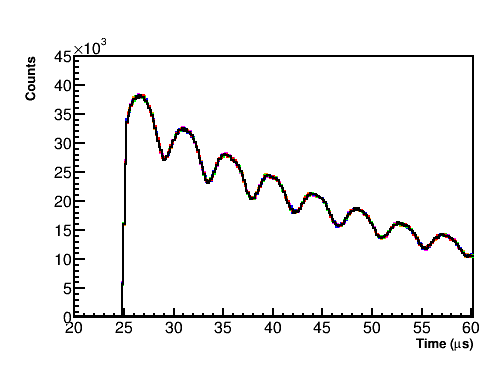
\includegraphics[width=\textwidth]{SDT_PileupTimeComparison_9d_auto}
        \caption{The pileup time spectrum for different choices of SDT.}
    \end{subfigure}% %you need this % here to add spacing between subfigures
    \hspace{1cm}
    \begin{subfigure}[t]{0.45\textwidth}
        \centering
        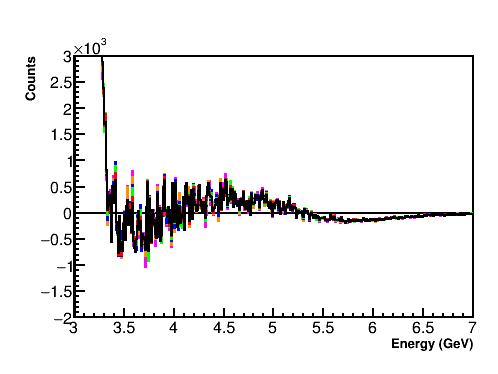
\includegraphics[width=\textwidth]{SDT_CorrEnergyComparison_9d_auto}
        \caption{The corrected energy spectrum for different choices of SDT.}
    \end{subfigure}
\caption[Pileup shadow dead time scan with automatic pileup amplitude scaling]{Shadow dead time scan results with automatic pileup amplitude scaling. No clear minimum is observed in the \chisq plot, and the sensitivity for $R$ is small. In the bottom two spectra plots the magenta curve corresponds to a choice SDT = \ns{5} while the black curve corresponds to SDT = \ns{10}. With the automatic amplitude scaling applied, the time and energy spectra are nearly identical and lie on top of each other. That combined with the lack of clear minimum in the \chisq plot and no clear sensitivity in $R$ indicate that there is no real systematic error due to the choice of SDT. Data from 9d dataset.}
\label{fig:SDTscan_autoScaling}
\end{figure}


In order to calculate the systematic dependence on the choice of SGT (default value of \ns{10}), the SGT parameter was scanned over from \ns{10} to \ns{20} in steps of \ns{1}. The results of the study with the automatic pileup amplitude scaling applied is shown in \figref{fig:SGTscan}. Just as in the SDT scan with the automatic pileup amplitude scaling, there is no minimum in the \chisq results, the sensitivity of $R$ to the value of SGT not so clear, and the pileup spectra for the various choices of SGT are nearly identical. Therefore again any systematic error due to the choice of SGT is subsumed into the pileup amplitude error.


\begin{figure}[]
\centering
    \begin{subfigure}[t]{0.45\textwidth}
        \centering
        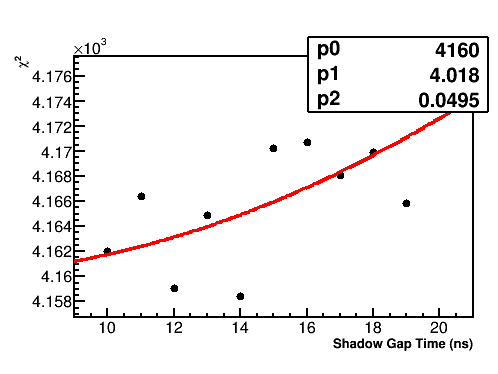
\includegraphics[width=\textwidth]{FullRatio_Chi2_Vs_ShadowGapTime_Canv_9d}
        \caption{\chisq versus SGT. The parabolic fit equation used was $y = p_{2}(x - p_{1})^{2} + p_{0}.$}
    \end{subfigure}% %you need this % here to add spacing between subfigures
    \hspace{1cm}
    \begin{subfigure}[t]{0.45\textwidth}
        \centering
        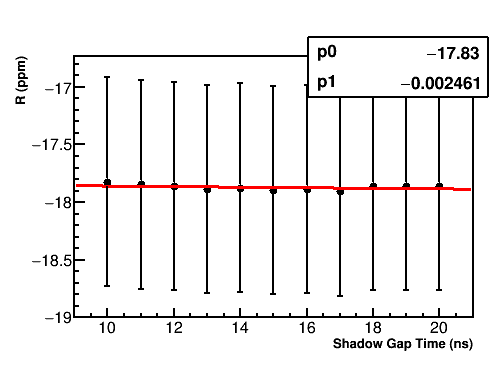
\includegraphics[width=\textwidth]{FullRatio_R_Vs_ShadowGapTime_Canv_9d}
        \caption{$R$ versus SGT. The parameter $p_{1}$ gives the sensitivity of $R$ to the value of SGT, with units in ppm/ns.}
    \end{subfigure}

    \begin{subfigure}[t]{0.45\textwidth}
        \centering
        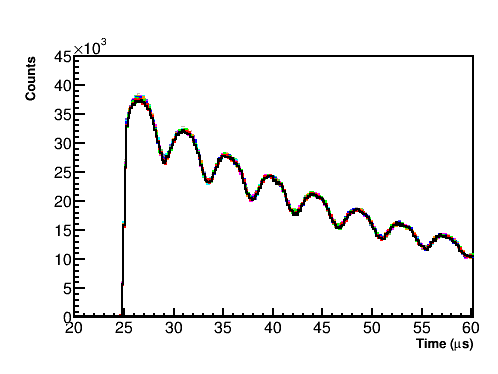
\includegraphics[width=\textwidth]{SGT_PileupTimeComparison_9d}
        \caption{The pileup time spectrum for different choices of SGT.}
    \end{subfigure}% %you need this % here to add spacing between subfigures
    \hspace{1cm}
    \begin{subfigure}[t]{0.45\textwidth}
        \centering
        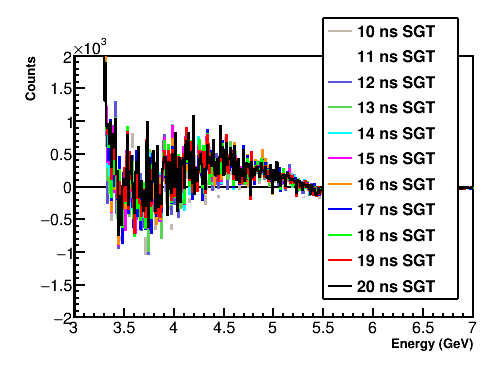
\includegraphics[width=\textwidth]{SGT_CorrEnergyComparison_9d}
        \caption{The corrected energy spectrum for different choices of SGT.}
    \end{subfigure}
\caption[Pileup shadow gap time scan with automatic pileup amplitude scaling]{Shadow gap time scan results with automatic pileup amplitude scaling. No clear minimum is observed in the \chisq plot, and the trend for $R$ isn't clear, with points fluctuating above and below the fit curve. In the bottom two spectra plots one of the grey curves (hidden) corresponds to a choice SGT = \ns{10} while the black curve corresponds to SGT = \ns{20}. With the automatic amplitude scaling applied, the time and energy spectra lie on top of each other. That combined with the lack of clear minimum in the \chisq plot and small sensitivity in $R$ indicate that there is no real systematic error due to the choice of SGT. Data from 9d dataset.}
\label{fig:SGTscan}
\end{figure}


The pileup amplitude systematic error is the error on $R$ assuming the scale of the pileup was incorrectly constructed. In order to evaluate this error, multipliers were applied to the pileup spectra from 0.9 to 1.1 in steps of 0.01 (dropping the default automatic pileup scaling of $\sim1.03$ mentioned before). The data was then re-fit to find the change in $R$. The results of the study for the 9d dataset are shown in \figref{fig:PMscan}. As shown there is a clear minimum near 1 in the \chisq results and a large sensitivity of $R$ to the multiplier. The systematic error on $R$ is calculated as 
    \begin{align}
        \delta R = \sigma_{P_{m}} \times \frac{dR}{dP_{m}},
    \end{align}
where $P_{m}$ is the value of the pileup multiplier. The error $\sigma_{P_{m}}$ is calculated as the width of the fitted parabola in the \chisq plot, defined as the change in $P_{m}$ from the minimum for the \chisq to increase by 1. This is calculated as 
    \begin{align}
        \sigma_{P_{m}} = \sqrt{\frac{2}{f''(\chi^{2})}} = \frac{1}{\sqrt{p_{2}}},
    \end{align}
where $p_{2}$ is the fit parameter as given in the top right of the \chisq plot. The sensitivities of $R$ to the pileup multiplier, uncertainties in the pileup amplitude, and final corresponding systematic errors for the Run~1 precession frequency analysis datasets are given in \tabref{tab:systematicError_pileupMultplier}. As shown in the table, the uncertainties on the pileup amplitude are of order 2 to 5\%, while the systematic errors on $R$ are on the order of \SI{10}{} to \SI{20}{ppb} depending on dataset.  It should be noted that the default automatic pileup multiplier of $\sim1.03$ does not necessarily correspond to the minimum in the \chisq plot, but is within $1\sigma$ of 1 or the minimum (except the Endgame which is closer to $2\sigma$)\footnote{Monte-Carlo tests with various random seeds showed this minimum fluctuating above and below 1. The distance from 1 therefore is not a good measure for the uncertainty in the pileup amplitude compared to the width of the \chisq parabola fit.}.


\begin{figure}[]
\centering
    \begin{subfigure}[t]{0.45\textwidth}
        \centering
        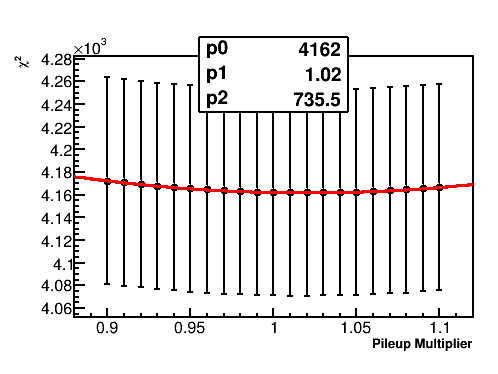
\includegraphics[width=\textwidth]{FullRatio_Chi2_Vs_PileupMultiplier_Canv_9d}
        \caption{\chisq versus pileup multiplier. The parabolic fit equation used was $y = p_{2}(x - p_{1})^{2} + p_{0}.$}
    \end{subfigure}% %you need this % here to add spacing between subfigures
    \hspace{1cm}
    \begin{subfigure}[t]{0.45\textwidth}
        \centering
        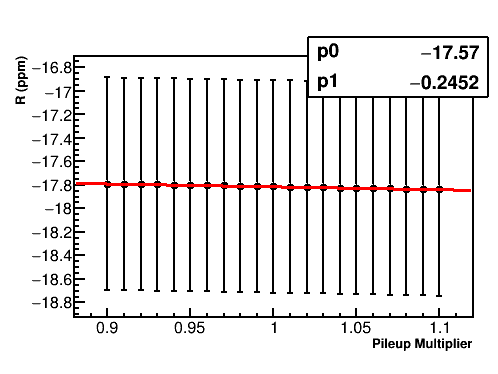
\includegraphics[width=\textwidth]{FullRatio_R_Vs_PileupMultiplier_Canv_9d}
        \caption{$R$ versus pileup multiplier. The parameter $p_{1}$ gives the sensitivity of $R$ to the value of the pileup multiplier, with units in ppm.}
    \end{subfigure}
\caption[Pileup multiplier scan]{Pileup multiplier scan. Data from 9d dataset.}
\label{fig:PMscan}
\end{figure}


\begin{table}[]
\centering
% \small
\setlength\tabcolsep{10pt}
\renewcommand{\arraystretch}{1.2}
\begin{tabular*}{0.65\linewidth}{@{\extracolsep{\fill}}lcccK}
% \begin{tabular}{@{\extracolsep{\fill}}lcccK}
  \hline
    \multicolumn{5}{c}{\textbf{Systematic Error due to Pileup Amplitude}} \\
  \hline\hline
    Dataset & \multicolumn{1}{c}{$dR/dP_{m}$} & $\sigma_{P_{m}}$ & $P_{m_{\text{min}}}$ & \multicolumn{1}{c}{$\boldsymbol{\delta R}$} \\
  \hline
    60h & $-419.3$ & 0.053 & 0.993 & 22.2 \\
    HighKick & $-372.8$ & 0.051 & 0.997 & 19.0 \\
    9d & $-245.2$ & 0.037 & 1.020 & 9.0 \\ 
    Endgame & $-335.3$ & 0.028 & 0.985 & 9.4 \\
  \hline
\end{tabular*}
\caption[Systematic error due to pileup amplitude]{Systematic error due to the pileup amplitude in the Ratio Method fits for the Run~1 precession frequency analysis datasets. The bold column gives the systematic error on \R. Units for $dR/dP_{m}$ and $\delta R$ are in ppb.}
\label{tab:systematicError_pileupMultplier}
\end{table}


The pileup phase error is the error on $R$ assuming the phase of the pileup was incorrectly constructed. This is separated into two parts. The first part is calculated by applying time-shifts to $t_{\text{doublet}}$ as given in \equref{eq:tdoublet}. Doing this artificially applies a phase shift to the pileup time spectrum. The data is then re-fit with the different pileup spectra and the change in $R$ is calculated. \figref{fig:PTSscan} shows the study results for the 9d dataset with time-shifts applied between \ns{-10} and \ns{10} in steps of \ns{1}. A clear sensitivity of $R$ to the value of time-shift is observed, however there is no clear minimum in the \chisq results. Because the width of the \chisq parabolic fit cannot be taken as the uncertainty in the pileup time-shift parameter , instead the uncertainty is taken conservatively at half the ADT at \ns{2.5}. The systematic error is calculated in the same way as for the pileup amplitude uncertainty,
    \begin{align}
        \delta R = \sigma_{P_{t}} \times \frac{dR}{dP_{t}},
    \end{align}
where $P_{t}$ is the value of the pileup time-shift. The sensitivities of $R$ to the pileup time-shift and corresponding systematic errors for the Run~1 precession frequency analysis datasets are given in \tabref{tab:systematicError_pileupTimeShift}.


\begin{figure}[]
\centering
    \begin{subfigure}[t]{0.45\textwidth}
        \centering
        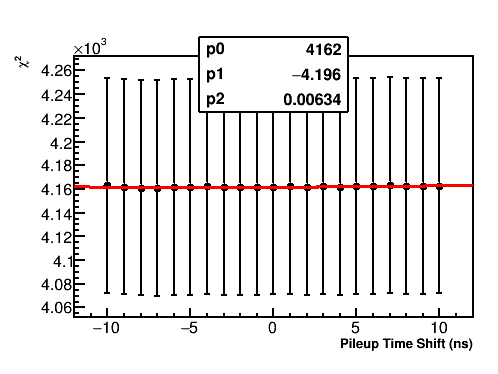
\includegraphics[width=\textwidth]{FullRatio_Chi2_Vs_PileupTimeShift_Canv_9d}
        \caption{\chisq versus pileup time-shift. There is no clear minimum in the plot.} 
    \end{subfigure}% %you need this % here to add spacing between subfigures
    \hspace{1cm}
    \begin{subfigure}[t]{0.45\textwidth}
        \centering
        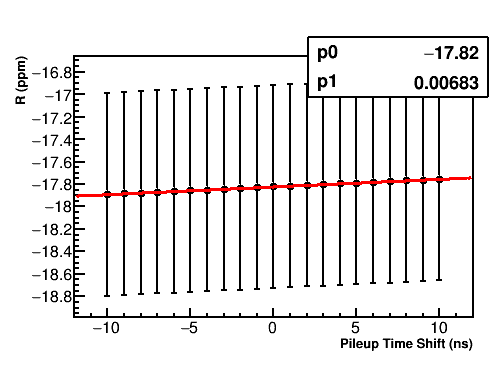
\includegraphics[width=\textwidth]{FullRatio_R_Vs_PileupTimeShift_Canv_9d}
        \caption{$R$ versus pileup time-shift. The parameter $p_{1}$ gives the sensitivity of $R$ to the value of the pile time-shift, with units in ppm/ns.}
    \end{subfigure}
\caption[Pileup time-shift scan]{Scan over pileup time-shift. Data from 9d dataset.}
\label{fig:PTSscan}
\end{figure}


\begin{table}[]
\centering
% \small
\setlength\tabcolsep{20pt}
\renewcommand{\arraystretch}{1.2}
\begin{tabular*}{0.7\linewidth}{@{\extracolsep{\fill}}lcK}
% \begin{tabular}{@{\extracolsep{\fill}}lcccK}
  \hline
    \multicolumn{3}{c}{\textbf{Systematic Error due to Pileup Time Shift}} \\
  \hline\hline
    Dataset & \multicolumn{1}{c}{$dR/dP_{t}$} & \multicolumn{1}{c}{$\boldsymbol{\delta R}$} \\
  \hline
    60h & 7.0 & 17.6 \\
    HighKick & 7.6 & 19.0 \\
    9d & 6.8 & 17.1 \\ 
    Endgame & 5.7 & 14.3 \\
  \hline
\end{tabular*}
\caption[Systematic error due to pilep time shift]{Systematic error due to the pileup time-shift parameter $P_{t}$ in the Ratio Method fits for the Run~1 precession frequency analysis datasets. The bold column gives the systematic error on \R. Units for $dR/dP_{t}$ and $\delta R$ are in ppb/ns and ppb respectively. The error on the $P_{t}$ is by default taken to be \ns{2.5} as described in the text. \textbf{fix spacing of table}}
\label{tab:systematicError_pileupTimeShift}
\end{table}


% -maybe put in fit start time scan of various time shifts converging to one
% -maybe add plot of nice energy threshold where pileup goes smooth and phase error would disappear


The second part of the pileup phase error comes from the choice of constant $C$ in the calculation of $E_{\text{doublet}}$ as given in \equref{eq:Edoublet}. If the energy of the pileup pulses are systematically mis-constructed, then pileup shadow doublets will be added or lost near the applied energy threshold when constructing the pileup spectrum. This leads to an error on the pileup phase since it is energy-dependent. In order to calculate the systematic error from the energy construction, the parameter $C$ was scanned over from 0.9 to 1.1, in steps of 0.01. The results of the study for the 9d dataset are shown in \figref{fig:PEscan}. The systematic error on $R$ is calculated as 
    \begin{align}
        \delta R = \sigma_{C} \times \frac{dR}{dC}.
    \end{align}
Similarly to the pileup amplitude error, there is a clear minimum in the \chisq results which can be used to estimate the uncertainty in the pileup energy scale\footnote{The trend isn't as clean as in the scan over the pileup amplitude multiplier, but that is acceptable.}. \tabref{tab:systematicError_pileupC} gives the sensitivities of $R$ to the pileup energy scale, uncertainties in the pileup energy scale, and the corresponding final systematic errors for the Run~1 precession frequency analysis datasets. As shown the uncertainties on the pileup energy scale are of order 1 to 2\%, and the value for $C$ which produces the minimum in the \chisq results is consistent with 1\footnote{Because the spatial separation is turned off in the clustering portion of the reconstruction, a value of $C = 1$ is to be expected.}. Interestingly, the sensitivity of $R$ to $C$ in the 60h dataset is noticeably larger than in the rest of the datasets, though the origin of this is currently unknown. \textbf{what to do about this?}


\begin{figure}[]
\centering
    \begin{subfigure}[t]{0.45\textwidth}
        \centering
        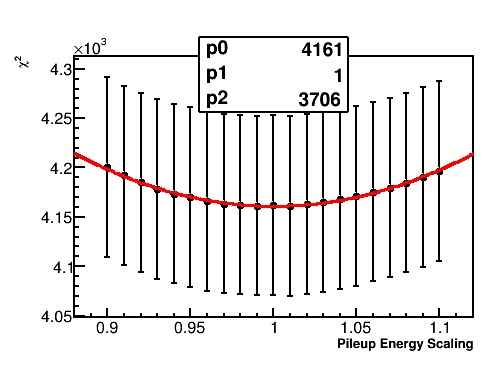
\includegraphics[width=\textwidth]{FullRatio_Chi2_Vs_PileupEnergyScaling_Canv_9d}
        \caption{\chisq versus pileup energy scale. The parabolic fit equation used was $y = p_{2}(x - p_{1})^{2} + p_{0}.$}
    \end{subfigure}% %you need this % here to add spacing between subfigures
    \hspace{1cm}
    \begin{subfigure}[t]{0.45\textwidth}
        \centering
        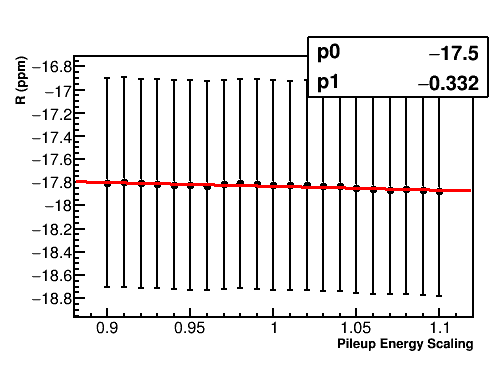
\includegraphics[width=\textwidth]{FullRatio_R_Vs_PileupEnergyScaling_Canv_9d}
        \caption{$R$ versus $C$. The parameter $p_{1}$ gives the sensitivity of $R$ to the value of $C$, with units in ppm.}
    \end{subfigure}
\caption[Pileup energy scale scan]{Scan over pileup energy scale. Data from 9d dataset.}
\label{fig:PEscan}
\end{figure}


\begin{table}[]
\centering
% \small
\setlength\tabcolsep{12pt}
\renewcommand{\arraystretch}{1.2}
\begin{tabular*}{0.65\linewidth}{@{\extracolsep{\fill}}lcccK}
% \begin{tabular}{@{\extracolsep{\fill}}lcccK}
  \hline
    \multicolumn{5}{c}{\textbf{Systematic Error due to Pileup Energy Scale}} \\
  \hline\hline
    Dataset & \multicolumn{1}{c}{$dR/dC$} & $\sigma_{C}$ & $C_{\text{min}}$ & \multicolumn{1}{c}{$\boldsymbol{\delta R}$} \\
  \hline
    60h & $-835.1$ & 0.023 & 0.997 & 19.4 \\
    HighKick & $-167.7$ & 0.022 & 0.995 & 3.7 \\
    9d & $-332.0$ & 0.016 & 1.000 & 5.5 \\ 
    Endgame & $-431.4$ & 0.012 & 0.982 & 5.3 \\
  \hline
\end{tabular*}
\caption[Systematic error due to fixed pileup energy scale factor]{Systematic error due to the fixed pileup energy scale parameter $C$ in the Ratio Method fits for the Run~1 precession frequency analysis. The bold column gives the systematic error on \R. Units for $dR/dC$ and $\delta R$ are in ppb.}
\label{tab:systematicError_pileupC}
\end{table}


\tabref{tab:PileupErrorsTotal} gives the quadrature sum for the total pileup systematic errors for the Run~1 precession frequency analysis datasets. As shown for each dataset the total error is below the target final error of \SI{40}{ppb} in spite of the contamination in the pileup shadow method. For future runs of the experiment with increased rate and therefore increased pileup, these errors may grow. In that case either the pileup shadow method might need to be improved to account for the contamination and pileup triplets, or discarded in favor of a different method.


\begin{table}[]
\centering
\setlength\tabcolsep{10pt}
\renewcommand{\arraystretch}{1.2}
\begin{tabular*}{\linewidth}{@{\extracolsep{\fill}}lcGGGG}
  \hline
    \multicolumn{6}{c}{\textbf{Total Pileup Systematic Errors}} \\
  \hline\hline
    Type of Error & Parameter & \multicolumn{1}{c}{60h} & \multicolumn{1}{c}{HighKick} & \multicolumn{1}{c}{9d} & \multicolumn{1}{c}{Endgame} \\
  \hline
    Amplitude & $P_{m}$  & 22.2 & 19.0 & 9.0  & 9.4 \\
    Phase     & $P_{t}$  & 17.6 & 19.0 & 17.1 & 14.3 \\
    Phase     & $C$      & 19.4 & 3.7  & 5.5  & 5.3 \\
  \hline
    Quadrature sum &  & 34.3 & 27.1 & 20.1 & 17.9 \\
  \hline 
\end{tabular*}
\caption[Total pileup systematic errors]{Total pileup systematic errors for the Run~1 precession frequency analysis datasets.}
\label{tab:PileupErrorsTotal}
\end{table}




\subsection{Gain systematic errors}
\label{sub:gainerror}


As described in \secref{sub:LaserCalibrationSystem}, the energies of the positron hits are gain-corrected for in-fill, short-term double pulse, and out-of-fill effects. The latter occurs over time scales much longer than a fill, and thus does not bias the precession frequency measurement. For the cases of in-fill or STDP gain variations, any uncorrected fluctuations in the gain causes acceptance changes over the course of a fill which then modifies the average measured phase of the detected positrons above threshold, and thus causes a systematic shift in the extracted $R$ value. 


The IFG function which describes the measured energies of the individual crystal hits as described in \secref{sec:ReconWest} is given by \cite{IFG}
    \begin{align} \label{eq:IFG}
        E = E_{0}(1 - C_{A} e^{-t/\tau_{g}}),
    \end{align}
where $E_{0}$ is the `true' energy of the detected positron and $E$ is the as-measured energy. Constants $C_{A}$ and $\tau_{g}$ are measured with the laser calibration system, and then the function given in \equref{eq:IFG} is used to convert the measured energies back to their real energies. In order to determine a systematic error from the applied IFG function, the IFG function was un-applied to the crystal hits before reapplying it with modified parameters. Specifically, the parameter $C_{A}$ was scanned over in multiplicative steps, such that all crystal energies included in a cluster hit were adjusted by some multiplicative factor before re-summing\footnote{It was decided that scanning over the parameter $\tau_{g}$ was unnecessary as it in general shifts the energies of the positrons in the same way as $C_{A}$.}. The multipliers applied to the IFG amplitude were \{0, 0.5, 1, 1.5, and 2\}. The results of the scan for the 60h dataset is shown in \figref{fig:IFG_amplitude}, with a comparison to the results from a T-Method fit. It is immediately apparent that the sensitivity of the T Method to the IFG multiplier is far greater than that of the Ratio Method. The Ratio Method's insensitivity to slowly varying effects which divide out is one of it's primary strengths. In fact, while there is an observable minimum in the T Method \chisq results, no such minimum exists in for the ratio fits.  


\begin{figure}[]
\centering
    \begin{subfigure}[]{0.45\textwidth}
        \centering
        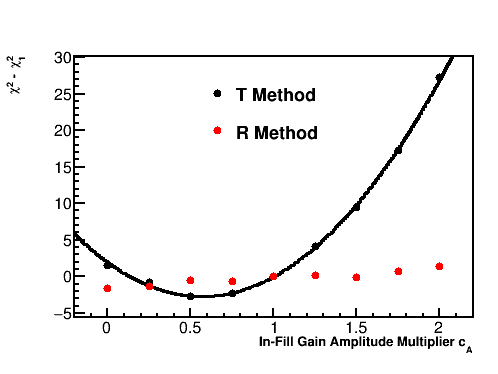
\includegraphics[width=\textwidth]{Chi2_Vs_IFG_Amp_crystals_compare_60h}
        \caption{Normalized \chisq vs IFG multiplier. The T Method points fit nicely to a parabolic curve while the Ratio Method points do not.}
    \end{subfigure}% %you need this % here to add spacing between subfigures
    \hspace{4mm}
    \begin{subfigure}[]{0.45\textwidth}
        \centering
        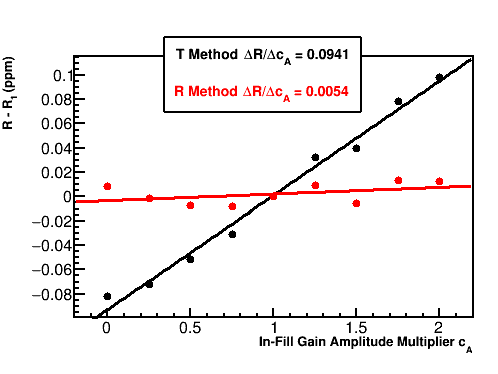
\includegraphics[width=\textwidth]{R_Vs_IFG_Amp_crystals_compare_60h}
        \caption{$R$ values vs IFG multiplier. Both points are fit to straight lines, and the slopes are included in the text box in units of ppm.}
    \end{subfigure}
\caption[]{Fitted \chisq's and $R$ values for the 60h dataset as a function of IFG amplitude multiplier. Results with ratio fits (red) are compared to T Method fits (black). Values are normalized to their $C_{A} = 1$ results in order to put the curves on the same scale. As shown the sensitivity in the T Method to the IFG amplitude is significantly larger than that in the Ratio Method. This is one of the primary strengths of the Ratio Method.}
\label{fig:IFG_amplitude}
\end{figure}


\tabref{tab:systematicError_IFG} gives the sensitivities of the T Method and R Method fits for all the datasets, along with the T Method minimum for $C_{A}$. There are some interesting things to observe when looking at all the values in the chart. The T Method values, while not the primary subject of this analysis, nevertheless vary between the datasets and especially for the minimums which are not consistent with one another. This implies there might be some very small gain correction imperfections which have not been fully accounted for. The confidence in the Ratio Method results is preserved from the fact that the Ratio Method fits are not as sensitive to the gain variations as the T Method. It should still be noticed however that there are some significantly varying sensitivities in the Ratio Method $R$ values to $C_{A}$, as evidence by the values for the HighKick and Endgame. For the Endgame dataset there was one fit point in particular at $C_{A} = 2$ which was noticeably different than the rest, which pulled the slope of $R/C_{A}$ up the value shown. For the HighKick dataset a negative slope was observed, with all points lying relatively consistent with one another with no outliers. The near-zero slopes of the 60h and 9d datasets give some implication that these slopes are all largely random which might save things. \textbf{I should do more fits to the gain just to double check values and make some more convincing curves - a lot of grid jobs and very annoying but I should just do it.} Though not included in the table \textbf{maybe I should include them?} the changes in $R$ with versus without the IFG function applied at all are less than \SI{10}{}, \SI{30}{}, \SI{5}{}, and \SI{10}{ppb} for the 60h, HighKick, 9d, and Endgame datasets respectively. \textbf{I should find these exact numbers and print them out - maybe after further gain fits} These values in general give an upper bound to any systematic effects that a mis-applied IFG function might cause. The uncertainties on the IFG amplitudes from fits to the laser data were in general of order 25\% \cite{AnnaPersonalComm}, which when multiplied against the Ratio Method $R$ sensitivities results in systematic errors of \SI{<6}{ppb} for the various dataset. The individual numbers are given in \tabref{tab:systematicError_IFG}.


-update text based on latest fits which ultimately didn't change the trends or interesting things I'm seeing


\begin{table}[]
\centering
% \small
% \setlength\tabcolsep{12pt}
\renewcommand{\arraystretch}{1.2}
\begin{tabular*}{1\linewidth}{@{\extracolsep{\fill}}lccGK}
% \begin{tabular}{@{\extracolsep{\fill}}lcccK}
  \hline
    \multicolumn{5}{c}{\textbf{Systematic Error due to IFG Amplitude}} \\
  \hline\hline
            & \multicolumn{1}{c}{T-Method} & \multicolumn{1}{c}{T-Method} & \multicolumn{1}{c}{R-Method} & \multicolumn{1}{c}{R-Method} \\
    Dataset & \multicolumn{1}{c}{$dR/dC_{A}$} & \multicolumn{1}{c}{$C_{A_{\text{min}}}$} & \multicolumn{1}{c}{$dR/dC_{A}$} & \multicolumn{1}{c}{$\boldsymbol{\delta R}$} \\
  \hline
    60h & 94.1 & 0.57 & 5.4 & 1.4 \\
    HighKick & 69.5 & 0.70 & -23.6 & 5.9 \\
    9d & 64.9 & 0.27 & 1.4 & 0.4 \\ 
    Endgame & 96.2 & 0.19 & 22.7 & 5.7 \\
  \hline
\end{tabular*}
\caption[Systematic error due to IFG amplitude]{Sensitivities and systematic errors related to the IFG amplitude. Also included are some T Method numbers for comparison. Units are in ppb.}
\label{tab:systematicError_IFG}
\end{table}



For the stdp....

\cite{STDP}





\subsection{CBO systematic errors}
\label{sub:cboerror}


If the CBO is mis-modeled then there will be a systematic error on $R$ since there is a an early-to-late change in both the frequency and the scale of the CBO. The CBO model is largely constrained by tracker measurements, but systematic errors can be evaluated by modifying the fixed frequency function described in \secref{sec:MuonBeamMeasurements} and given in \equref{eq:CBOfreqForm}, and the decoherence envelope of the CBO.

\tabref{tab:CBOFrequencyParameters} gives the CBO frequency model parameters for both tracker stations. The station 12 values are by default used in all fits to the data. Fits were performed with the station 18 values, the changes in $R$ are given in \tabref{tab:systematicError_Station18}. The absolute values of the changes for the different datasets are conservatively taken as the systematic error on $R$ due to the choice of fixed CBO frequency model parameters. While the CBO parameters in the tracking analysis fits do have errors on the parameters, they are tiny compared to the systematic errors between the two tracker stations \cite{CBOFreqTrackingElog}. Some few fits were made by varying the fixed frequency parameters by $1\sigma$ in there errors, and the changes in $R$ were negligible. For this reason the systematic errors from using station 18 values is taken as the error.



\begin{table}[]
\centering
% \small
% \setlength\tabcolsep{10pt}
\renewcommand{\arraystretch}{1.2}
\begin{tabular*}{0.75\linewidth}{@{\extracolsep{\fill}}lH}
  \hline
    \multicolumn{2}{c}{\textbf{Change in $R$ with station 18 CBO parameters}} \\
  \hline\hline
    Dataset & \multicolumn{1}{c}{$\boldsymbol{\delta R}$} \\
  \hline
    60h & 7.5 \\
    HighKick & 0.4 \\
    9d & -2.0 \\
    Endgame & 8.0 \\
  \hline
\end{tabular*}
\caption[Changes in $R$ with tracker station 18 CBO frequency model parameters]{Changes in the fitted $R$ values with tracker station 18 CBO frequency model parameters instead of tracker station 12. The systematic errors are conservatively taken as the absolute value in the changes in $R$. Units are in ppb.}
\label{tab:systematicError_Station18}
\end{table}


The shape of the CBO, or the decoherence envelope, is also similarly constrained by the tracking analysis. The envelope is typically by default an exponential as given in \equref{eq:Ncbo} and shown in \figref{fig:CBOAmplitude}. The only other envelope which could reasonably exist in the data is an exponential plus a constant
    \begin{align}
        e^{-t/\boldsymbol{\tau_{cbo}}} \rightarrow e^{-t/\boldsymbol{\tau_{cbo}}} + C,
    \end{align}
where $C$ is some constant CBO amplitude which lives over the course of each fill. In order to assess this systematic error, this new envelope was introduced into the $N_{cbo}(t)$ fit term. Fits were done with $C$ floating, where the starting value for $C$ was taken from a T Method fit to the data. While in T Method fits the $C$ parameter converged to values with errors about half the value, in general in the Ratio Method fits the $C$ parameters had relatively large errors. In spite of the large errors however, the fits converged properly with the floating $C$ parameter. In general the final fit parameters are largely the same, with the exception being the fitted CBO lifetime which about halves. This is unsurprising as the lifetime is highly correlated to the amplitude. Only in the 9d dataset did some small complications arise, where the CBO lifetime had to be fixed in order to get the fit to converge properly, and even with being fixed the $C$ parameter converged to a negative value. The fitted values for the $C$ constants and the changes in the final fitted $R$ values are given in \tabref{tab:systematicError_CBOEnvelope}. As shown the changes in $R$ are of order 10s of ppb for some of the datasets, with $R$ varying both positively and negatively. These changes in $R$ are conservatively taken as the systematic errors on $R$ for the different datasets.



\begin{table}[]
\centering
% \small
% \setlength\tabcolsep{10pt}
\renewcommand{\arraystretch}{1.2}
\begin{tabular*}{0.75\linewidth}{@{\extracolsep{\fill}}lGGG}
  \hline
    \multicolumn{4}{c}{\textbf{Systematic Error due to CBO Envelope}} \\
  \hline\hline
    Dataset & \multicolumn{1}{c}{$C \times 10^{-4}$} & \multicolumn{1}{c}{$\sigma_{C} \times 10^{-4}$} & \multicolumn{1}{c}{$\boldsymbol{\delta R}$} \\
  \hline
    60h & 10.7 & 8.3 & 17.6 \\
    HighKick & 11.6 & 10.4 & -18.0 \\
    9d & -13.5 & 12.2 & 28.7 \\
    Endgame & 10.7 & 4.0 & -4.3 \\
  \hline
\end{tabular*}
\caption[Systematic error due CBO envelope]{Systematic error on $R$ due to the choice of CBO envelope. The fitted floating parameter $C$ and it's error are given along with the change in $R$ compared to the standard exponential envelope in units of ppb. The 9d dataset interestingly converges to a negative value for the CBO envelope which requires more study to fully understand.}
\label{tab:systematicError_CBOEnvelope}
\end{table}



-put here a paragraph on the end for the total cbo error just like I did with the pileup






\subsection{Lost muon systematic errors}
\label{sub:lostmuonserror}


As mentioned in \secref{subsec:lostmuons}, the triples spectrum is made with cuts as defined in \tabref{tab:lostmuoncuts}. Various backgrounds are subtracted off the triples spectrum in order to generate a clean sample of lost muons. \tabref{tab:lostmuonsvariousfits} gives the change in \R for various sets of cuts and background subtractions for the 9d and Endgame datasets. As shown the various different backgrounds and cuts ultimately make very little difference in the final fitted \R value. Similarly, stable beam contaminants in the form of deuterons and protons contaminate the lost muon spectrum. The former are largely removed by straightforward \DT and $\Delta t_{13}$ cuts. The latter can be mostly removed by cutting on the negative side of the $\Delta t_{13}$ distribution which separates the populations more readily, \figref{fig:deltaT13}, with $\Delta t_{13} \leq \SI{12.5}{ns}$. While this does largely remove the protons at the cost of statistics, the fitted \K parameter simply grows larger to compensate. Ultimately the effect on \R is negligible, with $\Delta R = \SI{-0.3}{ppb}$. The sum of these separate types of errors is conservatively taken at \SI{1}{ppb} for all datasets\footnote{For the T-Method fits, though the changes in \R are noticeably larger with the various cuts, they are still the same order of magnitude and the error is conservatively below \SI{1}{ppb}.}.


\begin{table}[]
\centering
\setlength\tabcolsep{10pt}
\renewcommand{\arraystretch}{1.2}
\begin{tabular*}{1\linewidth}{@{\extracolsep{\fill}}lcccc}
  \hline
    \multicolumn{5}{c}{\textbf{$\Delta R$ with Various Lost Muon Cuts}} \\
  \hline\hline
    & \multicolumn{2}{c}{9d Dataset} & \multicolumn{2}{c}{Endgame Dataset} \\
  \hline
    Type of fit or cut & $\Delta R$ (ppb) & \K & $\Delta R$ (ppb) & \K \\
  \hline
    No quadruple subraction & 0.2 & 1.811 & -0.1 & 1.717 \\
    No accidental subraction & 0.1 & 2.503 & $<0.1$ & 2.339 \\
    $\Delta t_{13} \leq \SI{12.5}{ns}$ & 0.1 & 4.469 & -0.3 & 4.248 \\
    $\SI{5}{ns} \leq \Delta t_{12, 23} \leq \SI{8.5}{ns}$ & N/A & N/A & $<0.1$ & 1.709 \\
    $\SI{100}{\MeV} \leq E_{1,2,3} \leq \SI{500}{\MeV}$ & N/A & N/A & $<0.1$ & 2.09 \\
  \hline 
\end{tabular*}
\caption[Effect on fitted R value due to lost muon cuts in the 9d and Endgame datasets]{Effect on the fitted \R value in the 9d and Endgame datasets with various different cuts used or backgrounds subtracted. Ultimately how the muon loss spectrum $L(t)$ is created has little bearing on the final fitted \R value. Also included are the various corresponding \K values which compensate for the level of statistics contained within $L(t)$ due to the various cuts. \textbf{decide whether to fill out the N/A 9d fits or not}}
\label{tab:lostmuonsvariousfits}
\end{table}


\begin{figure}[]
    \centering
    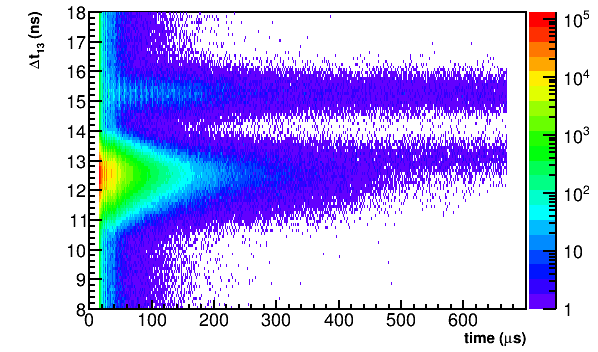
\includegraphics[width=.8\textwidth]{deltaT13_timeInFill_noCuts_Endgame}
    \caption[Lost muon $\Delta t_{13}$ distribution as a function of time in-fill]{Lost muon $\Delta t_{13}$ distribution as a function of time in-fill.}
    \label{fig:deltaT13}
\end{figure}



Of more interest is the choice of fixed value for the \K parameter in the ratio fits, fixed from the corresponding T-Method fits. The systematic error can be determined by simply scanning over the value of \K as in \figref{fig:kappaLossScan}, where the error on the parameter is that taken from a T-Method fit to the same data\footnote{The size of the error on \K is entirely due to statistics.}. \tabref{tab:systematicError_kappaLoss} gives the systematic errors on \R for the Run~1 precession frequency analysis datasets. Interestingly enough, though the Endgame dataset has the most lost muons, it is seen that the change in \R versus \K is larger in the other datasets. This is potentially due to the fact that \textbf{try to come up with something for this unless I can explain it away as an oddity.}


\begin{figure}[]
    \centering
    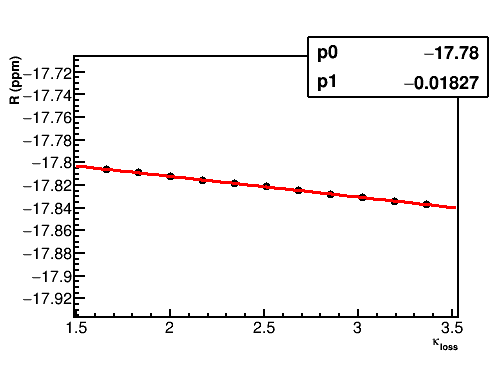
\includegraphics[width=.7\textwidth]{FullRatio_R_Vs_kappa_loss_Canv_9d}
    \caption[Scan over fixed \K]{The sensitivity of \R to the fixed \K parameter. Error bars have been removed from the plot. Units are in ppm, data from the 9d dataset.}
    \label{fig:kappaLossScan}
\end{figure}


\begin{table}[]
\centering
% \small
% \setlength\tabcolsep{10pt}
\renewcommand{\arraystretch}{1.2}
\begin{tabular*}{0.75\linewidth}{@{\extracolsep{\fill}}lGcJG}
  \hline
    \multicolumn{5}{c}{\textbf{Systematic Error due to Fixed $\kappa_{loss}$}} \\
  \hline\hline
    Dataset & \multicolumn{1}{c}{$dR/d\kappa_{loss}$} & $\sigma_{\kappa_{loss}}$ & \multicolumn{1}{c}{$\boldsymbol{\delta R}$} & \multicolumn{1}{c}{$\Delta R$ (with - without)} \\
  \hline
    60h & -3.5 & 0.338 & 1.2 & -31.4 \\
    HighKick & -7.1 & 0.697 & 4.9 & -40.1 \\
    9d & -18.3 & 0.170 & 3.1 & -45.7 \\
    Endgame & -2.6 & 0.038 & 0.1 & -6.1 \\
  \hline
\end{tabular*}
\caption[Systematic error due to fixed $\kappa_{loss}$]{Systematic error due to the fixed $\kappa_{loss}$ parameter in the Ratio Method fits for the Run~1 precession frequency analysis datasets. The bold column gives the systematic error on \R. The last column on the right gives the change in \R with the lost muons term included versus without, providing an absolute upper bound on systematic error. All units are in ppb except for the $\sigma_{\kappa_{loss}}$ parameter which is unit-less and comes from the T-Method fits.}
\label{tab:systematicError_kappaLoss}
\end{table}




- a systematic error comes from the fact that muons are lost preferentially at earlier times (changing over the course of a fill)
-if lost muons originate from different points in the beam line, then they will have precessed a different amount leading to a different phase


-this error dominates the uncertainty...


-probably move losses fraction figure to here somewhere


The fractional losses (the integral in \equref{eq:lambdalosses} times the final fitted $\kappa_{loss}$ parameter) for the Run~1 precession frequency analysis datasets are shown in \figref{fig:fractionallosses}.



\begin{figure}[]
    \centering
    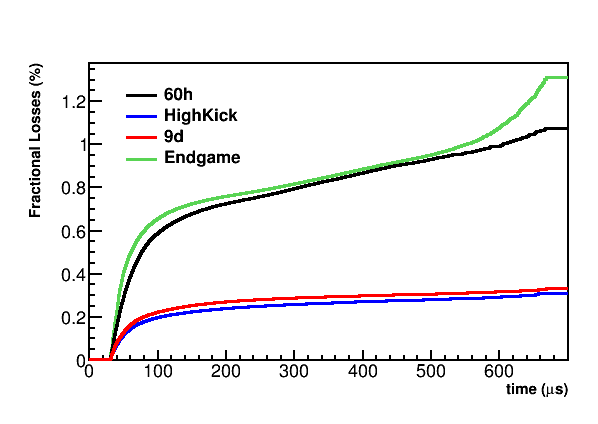
\includegraphics[width=.8\textwidth]{fractionalLosses_dataset_comparison}
    \caption[Fractional muon losses in the analyzed Run~1 datasets]{Fractional losses for the Run~1 precession frequency analysis datasets. The curves begin at \mus{30.2} which is where the fit begins. A value of 1\% at a specific time $t$ indicates that there are 1\% fewer stored muons at that time than there would be if there were no losses at all. The Endgame and 60h datasets can be seen to have the most losses, while the 9d and HighKick have less. This is due to the higher kicks in the latter datasets which put the muon beam on a more central orbit. The upward tail at the end of the Endgame dataset corresponds to the remnant proton contamination.}
    \label{fig:fractionallosses}
\end{figure}






-also Sudeshna's talk in the Elba collaboration meeting - this probably just for the systematic error






-put in a chart at the end summarizing the total lost muons systematic error - unless I want to keep the pieces separate, and have one giant chart at the end which might be too much



\subsection{Ratio construction systematic errors}
\label{sub:TimeShiftingParameters}

In the construction of the ratio data, when filling the four sub-datasets as in \equref{eqn:fourHistsInText}, the parameters $T_{a}$ and $\tau_{\mu}$ for the \gmtwo period and muon lifetime need to be known a priori. If these parameters are incorrectly chosen, then there will be a systematic shift on $R$. This is especially important when considering $T_{a}$, because the quantity which the E989 experiment is measuring must be used in the analysis, creating sort of a self-dependence. The question then naturally arises as to how well the $T_{a}$ parameter needs to be known. As described in \secref{sub:ratio_method}, the input value for $T_{a}$ is nominally taken as the result from the E821 experiment. 

In order to determine systematic errors from these two fixed quantities, they were scanned over when forming the ratio data before fitting. The input value for $T_{a}$ was varied from \SI{-30}{ppm} to \SI{+30}{ppm} around the default value in steps of \SI{3}{ppm}. The input value for $\tau_{\mu}$ was varied from \SI{64.04}{\micro s} to \SI{64.84}{\micro s} in steps of \SI{0.04}{\micro s}. See \figref{fig:ratioConstructionParsScan} for scan results for the 60h dataset. See \tabref{tab:ratioConstructionParsScan} for the sensitivities determined from the scans for all datasets. As shown the sensitivities vary both positively and negatively for the different datasets, and are extremely small. The positive and negative variations imply there is no real systematic effect at play, and that as long as a reasonable choice for these two parameters is made, then the ratio data is very insensitive to the exact values chosen. 

In order to be conservative however, a scale for the changes in $R$ is given. Since the measured \gmtwo period in the data is already modified by the hardware blinding, it is technically the hardware shifted \gmtwo period that we want to use. The calorimeter digitizers use a ``40'' MHz clock which has been blinded to a value in the range of 39.997 to \SI{39.999}{MHz}\cite{ClockManual}. This corresponds to a 75 ppm range in the frequency, in a uniform distribution. Calculating the uncertainty from the uniform distribution and adding it in quadrature with a conservative \SI{10}{ppm} uncertainty in the guess on the true \gmtwo period from the E821 result, 
            \begin{align}
                \delta T_{a} = \sqrt{(75)^{2}/12 + 10^{2}} = \SI{23.8}{ppm}.
            \end{align}
This results in a change in $R$ on the order of \SI{2.4}{ppb} for the 60h and HighKick datasets, and less for the 9d and Endgame datasets. Because this is so small and because the sensitivities vary positively and negatively, any systematic error from this quantity can reasonable be said to not exist.

Similarly, the sensitivities of $R$ to the chosen muon lifetime are very small, order \SI{}{ppb/ \micro s}. Since the uncertainties in the muon lifetime are of order \ns{}, any systematic errors from this parameter would be completely negligible even if the sensitivities all had the same sign.


\begin{figure}[]
\centering
    \begin{subfigure}[t]{0.45\textwidth}
        \centering
        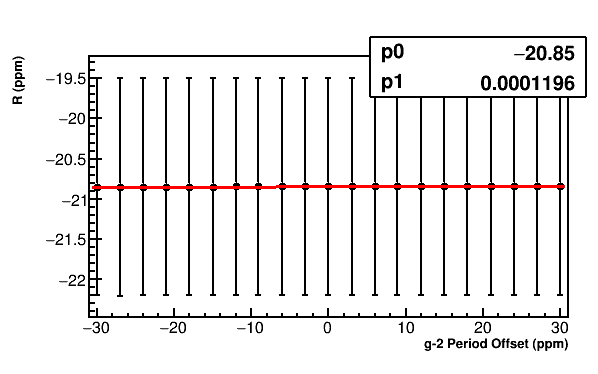
\includegraphics[width=\textwidth]{FullRatio_R_Vs_gm2PeriodGuess_Canv_60h}
        \caption{$R$ versus input value for $T_{a}$, where the x axis is given in units of a ppm level shift of the default choice for $T_{a}$.}
    \end{subfigure}% %you need this % here to add spacing between subfigures
    \hspace{4mm}
    \begin{subfigure}[t]{0.45\textwidth}
        \centering
        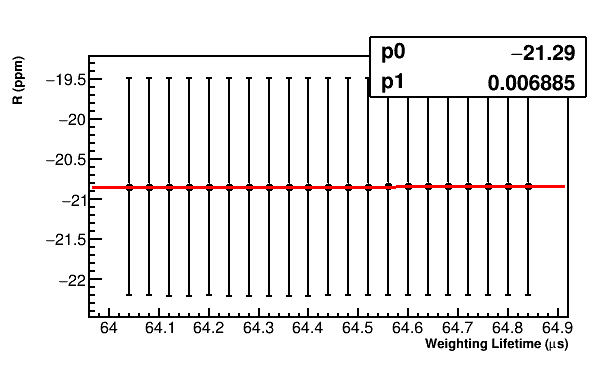
\includegraphics[width=\textwidth]{FullRatio_R_Vs_weightingLifetime_Canv_60h}
        \caption{$R$ versus the input value for $\tau_{\mu}$. Parameter $p_{1}$ gives the sensitivity in \SI{}{ppm/ \micro s}.}
    \end{subfigure}
\caption[Scans over ratio construction parameters]{Scans over ratio construction parameters for the 60h dataset. Error bars have been removed from the plots. In general the points are randomly spread around, and sensitivities are very small.}
\label{fig:ratioConstructionParsScan}
\end{figure}


\begin{table}[]
\centering
% \small
\setlength\tabcolsep{20pt}
\renewcommand{\arraystretch}{1.2}
\begin{tabular*}{0.7\linewidth}{@{\extracolsep{\fill}}lHH}
% \begin{tabular}{@{\extracolsep{\fill}}lcccK}
  \hline
    \multicolumn{3}{c}{\textbf{Sensitivity to Ratio Construction Parameters}} \\
  \hline\hline
    Dataset & \multicolumn{1}{c}{$dR/d_{T_{a}}$} & \multicolumn{1}{c}{$dR/d_{\tau_{\mu}}$} \\
  \hline
    60h & 0.1 & 6.9 \\
    HighKick & -0.1 & -4.1 \\
    9d & <0.1 & -1.1 \\ 
    Endgame & <0.1 & 0.6 \\
  \hline
\end{tabular*}
\caption[Sensitivities of $R$ to ratio construction parameters]{Sensitivities of $R$ to ratio construction parameters. $dR/d_{T_{a}}$ is in units of ppb/ppm, while $dR/d_{\tau_{\mu}}$ is in units of \SI{}{ppb/ \micro s}. In both cases the sensitivities are both extremely small, and vary negatively and positively for the different datasets. \textbf{fix spacing of table}}
\label{tab:ratioConstructionParsScan}
\end{table}






\subsection{Binning systematic errors}


When constructing the time spectra to be fit, bin widths and the starting edge of the bin are by default chosen to be \SI{149.2}{ns} and \SI{0}{ns} respectively. In order to verify that no systematics arise from the choice of these parameters, the values were scanned over. The bin width was scanned from \SI{148.7}{ns} to \SI{149.7}{ns} in steps of \SI{0.1}{ns}, while the bin edge was scanned from \SI{0}{ns} to \SI{149.2}{ns} in steps of \SI{14.92}{ns}. \figref{fig:binParametersScan} shows scan results for the 9d dataset. \tabref{tab:binParametersScan} gives the sensitivities of $R$ to both parameters. 

Upon general inspection of the fit points themselves, it was found that the trends weren't so convincing as the points varied relatively widely. Still a line was fit to the points to asses the scale of the changes. For the bin edge scan, it was verified that a shift of one bin width returned the same fit results as the default shift of \ns{0}. This combined with the negligible sensitivities and varying points implies no systematic effects on $R$ from the choice of bin edge. For the sensitivities to the choice of bin width, not only did the points vary, but the trends were both positive and negative depending on the dataset. In general the choice of bin width should be optimized to be equal to the peak of the cyclotron period distribution of the stored muons, which from the fast rotation analysis informed the choice of \SI{149.2}{ns} \cite{fastrotationsomething}. Therefore it is reasonable to quote no systematic error for the choice of bin width. If one wanted to be conservative and quote a systematic error however, the sensitivities could be multiplied against the uncertainty in the optimal bin width. This uncertainty from the fast rotation analysis is of order \SI{0.1}{ns}, which would correspond to uncertainties of \SI{2.5}{}, \SI{0.6}{}, \SI{2.3}{}, and \SI{4.2}{ppb} for the 60h, HighKick, 9d, and Endgame datasets respectively, all of which are practically negligible.



\begin{figure}[]
\centering
    \begin{subfigure}[t]{0.45\textwidth}
        \centering
        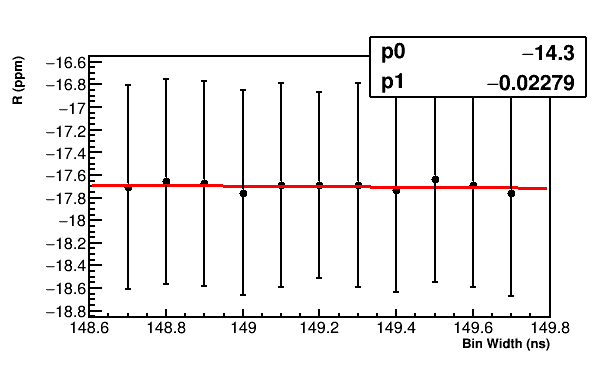
\includegraphics[width=\textwidth]{FullRatio_R_Vs_binWidth_Canv_9d}
        \caption{}
    \end{subfigure}% %you need this % here to add spacing between subfigures
    \hspace{1cm}
    \begin{subfigure}[t]{0.45\textwidth}
        \centering
        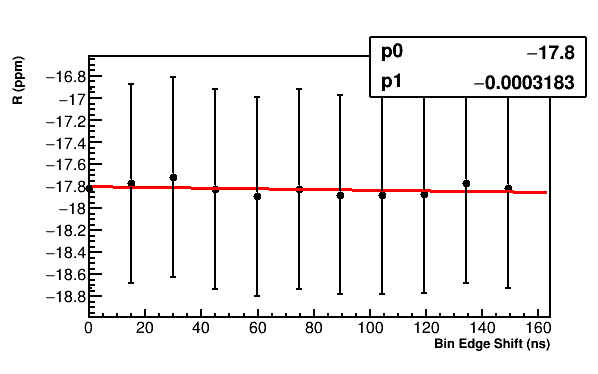
\includegraphics[width=\textwidth]{FullRatio_R_Vs_binEdgeShift_Canv_9d}
        \caption{}
    \end{subfigure}
\caption[Scans over binning parameters]{Scans over binning parameters for the 9d dataset. In general the points are randomly spread around, indicating no real systematic effect.}
\label{fig:binParametersScan}
\end{figure}


\begin{table}[]
\centering
% \small
\setlength\tabcolsep{20pt}
\renewcommand{\arraystretch}{1.2}
\begin{tabular*}{0.7\linewidth}{@{\extracolsep{\fill}}lGG}
% \begin{tabular}{@{\extracolsep{\fill}}lcccK}
  \hline
    \multicolumn{3}{c}{\textbf{Sensitivity to Binning Parameters}} \\
  \hline\hline
    Dataset & \multicolumn{1}{c}{$dR/d_{\text{bin width}}$} & \multicolumn{1}{c}{$dR/d_{\text{bin edge}}$} \\
  \hline
    60h & 24.5 & -0.1 \\
    HighKick & 6.0 & -0.7 \\
    9d & -22.8 & -0.3 \\ 
    Endgame & -41.7 & -0.6 \\
  \hline
\end{tabular*}
\caption[Sensitivities of $R$ to binning parameters]{Sensitivities of $R$ to binning parameters. Units are in ppb/ns. While some of these values may appear significant, inspection of the actual plots reveals that the actual trends are not quite so convincing. \textbf{fix spacing of table}}
\label{tab:binParametersScan}
\end{table}



\subsection{Systematics errors in the E field and pitch corrections}



\subsection{Systematic error summary}

-include here a big table (with each of the individual errors making up say pileup and the like) of all systematic errors



\begin{table}[]
\centering
% \small
% \setlength\tabcolsep{10pt}
\renewcommand{\arraystretch}{1.2}
\begin{tabular*}{\linewidth}{@{\extracolsep{\fill}}lcccc}


  \hline
    \multicolumn{5}{c}{\textbf{Systematic Errors}} \\
  \hline\hline
    Error & 60h & HighKick & 9d & Endgame \\ 
  \hline
    Pileup amplitude & & & & \\
    Pileup phase - time-shift & & & & \\
    Pileup phase - energy-scale & & & & \\
    In-fill gain amplitude & & & & \\
    STDP On/Off & & & & \\
    CBO frequency model & & & & \\
    CBO envelope & & & & \\
    Lost muon cuts & & & & \\
    Lost muon phase bias & & & & \\
    Ratio construction $T_{a}$ & & & & \\
    Ratio construction $T_{\mu}$ & & & & \\
    Bin width & & & & \\
    E field correction & & & & \\
    Pitch correction & & & & \\
  \hline
    Quadruature Sum & & & & \\
  \hline
\end{tabular*}
\caption[]{should I put all scan results here even if the conclusion was that there was no systematic error associated?}
\label{tab:}
\end{table}



